\documentclass[a4paper,12pt]{article}
\usepackage{url}
\usepackage[utf8]{inputenc}
\usepackage[T1]{fontenc}
\usepackage[brazilian]{babel}
\usepackage{graphicx}
\usepackage{subcaption}
\usepackage{amsmath}
\usepackage{geometry}
\usepackage{float}
\usepackage{booktabs}
\usepackage{caption}

\captionsetup{justification=centering}
\geometry{a4paper, margin=1in}
\renewcommand{\baselinestretch}{1.5}

\begin{document}
\thispagestyle{empty}

% ----------------------- CAPA -----------------------
\begin{center}
    \textbf{INSTITUTO FEDERAL DO ESPÍRITO SANTO}\\
    \textbf{CURSO DE ENGENHARIA ELÉTRICA}
\end{center}

\vspace{6cm}

\begin{center}
\textbf{Leandro Baldan Ferreira}\\
\textbf{Urilo Fabri}
\end{center}

\vspace{2cm}

\begin{center}
    \textbf{Projeto Final — Aprendizado de Máquina}
\end{center}

\vfill

\begin{center}
    Vitória\\
    2026
\end{center}

\newpage
\thispagestyle{empty}

\begin{center}
\textbf{Leandro Baldan Ferreira}\\
\textbf{Urilo Fabri}
\end{center}

\vspace{4cm}
\begin{center}
\textbf{\LARGE Classificação de Transações Bancárias com\\Técnicas de Aprendizado de Máquina}
\end{center}

\vspace{5cm}
\hspace{7cm}
\parbox{8cm}{
\small
Relatório apresentado à disciplina de Aprendizado de Máquina, do curso de Engenharia Elétrica do Instituto Federal do Espírito Santo, como requisito parcial para avaliação.\\
\newline
Prof.ª Dr.ª Mariana Rampinelli Fernandes
}

\vfill{}
\begin{center}
Vitória \\
2026
\end{center}

\newpage
\tableofcontents
\newpage

% ----------------------- INTRODUÇÃO -----------------------
\section{Introdução}

Este relatório apresenta o desenvolvimento de um projeto de classificação binária aplicado ao desafio \textit{Santander Customer Transaction Prediction}, disponível na plataforma Kaggle. O objetivo é prever se um cliente realizará uma transação futura, independentemente do valor transacionado, utilizando exclusivamente técnicas de aprendizado de máquina abordadas em aula.

O conjunto de dados disponibilizado pelo Santander contém 200.000 amostras de treinamento e 200.000 amostras de teste, cada uma composta por 200 atributos numéricos anônimos (denominados \texttt{var\_0} a \texttt{var\_199}). A métrica de avaliação oficial é a \textbf{Área Sob a Curva ROC} (AUC-ROC), que mede a capacidade do modelo de separar as classes sem depender de um limiar fixo de decisão.

Foram implementados e comparados três modelos com paradigmas distintos: \textbf{Random Forest}, \textbf{Naive Bayes Gaussiano} e \textbf{Support Vector Machine (SVM)} com kernel RBF. O projeto abrange as etapas de análise exploratória, pré-processamento, treinamento com validação cruzada estratificada e análise comparativa dos resultados.

\newpage

% ----------------------- DESCRIÇÃO DO PROBLEMA -----------------------
\section{Descrição do Problema}

\subsection{Conjunto de dados}

O conjunto de dados é composto por:

\begin{itemize}
    \item \textbf{Treino:} 200.000 amostras com 202 colunas (\texttt{ID\_code}, \texttt{target} e \texttt{var\_0} a \texttt{var\_199});
    \item \textbf{Teste:} 200.000 amostras com 201 colunas (sem \texttt{target});
    \item \textbf{Features:} 200 atributos numéricos contínuos completamente anônimos;
    \item \textbf{Valores ausentes:} nenhum.
\end{itemize}

\subsection{Desbalanceamento de classes}

O conjunto de treinamento apresenta 20.098 amostras positivas (target = 1) em um total de 200.000, correspondendo a aproximadamente \textbf{10\% de amostras positivas}. Trata-se de um desbalanceamento moderado, comum em problemas de detecção de transações, que exige cuidado na avaliação do modelo. A acurácia isolada, nesse contexto, pode ser enganosa, pois um classificador que sempre prevê a classe negativa obteria 90\% de acurácia sem detectar nenhuma transação real.

\subsection{Métrica de avaliação}

A métrica oficial do desafio é a \textbf{AUC-ROC}, definida como a área sob a curva que relaciona a Taxa de Verdadeiros Positivos (TVP) com a Taxa de Falsos Positivos (TFP) para diferentes limiares de decisão. Valores próximos de 1 indicam excelente capacidade discriminativa; valores próximos de 0,5 indicam desempenho equivalente ao acaso.

\newpage

% ----------------------- PRÉ-PROCESSAMENTO -----------------------
\section{Pré-processamento}

O pré-processamento foi implementado em um script dedicado (\texttt{preprocessing.py}), separado do treinamento dos modelos. Essa separação garante que a transformação dos dados seja realizada uma única vez e de forma consistente entre todos os modelos, evitando reprocessamentos desnecessários e possíveis inconsistências.

O fluxo executado pelo script é:

\begin{enumerate}
    \item Carregamento dos dados brutos;
    \item Verificação de qualidade;
    \item Padronização das features;
    \item Geração da subamostra para o SVM;
    \item Exportação dos arrays prontos para o treinamento.
\end{enumerate}

\subsection{Verificação de qualidade}

Antes de qualquer transformação, foram verificados:

\begin{itemize}
    \item \textbf{Valores ausentes:} nenhum ausente identificado no treino ou no teste;
    \item \textbf{Features constantes:} nenhuma feature apresentou valor único para todas as amostras;
    \item \textbf{Distribuição do target:} 20.098 positivos em 200.000 amostras (10,0\%), confirmando desbalanceamento moderado.
\end{itemize}

\subsection{Padronização}

Todos os atributos foram padronizados com média zero e desvio padrão unitário por meio do \texttt{StandardScaler}:

\[
x_{\text{pad}} = \frac{x - \mu}{\sigma}
\]

A padronização é obrigatória para o SVM, pois esse algoritmo é sensível à escala dos atributos — features com maior amplitude dominariam o cálculo da margem. Para o Naive Bayes Gaussiano, a padronização favorece a estimativa das distribuições por classe. O \textit{scaler} foi ajustado exclusivamente nos dados de treino e aplicado ao conjunto de teste, evitando vazamento de informação (\textit{data leakage}).

\subsection{Tratamento do desbalanceamento}

O parâmetro \texttt{class\_weight='balanced'} foi utilizado nos modelos Random Forest e SVM. Esse parâmetro ajusta automaticamente os pesos das classes de forma inversamente proporcional à sua frequência. O Naive Bayes Gaussiano não utiliza esse parâmetro, mas trata o desbalanceamento implicitamente pela estimativa da probabilidade a priori $P(C)$ a partir da frequência real das classes no conjunto de treino.

\[
w_c = \frac{n}{k \cdot n_c}
\]

onde $n$ é o número total de amostras, $k$ é o número de classes e $n_c$ é o número de amostras da classe $c$. Com isso, o modelo penaliza mais os erros na classe minoritária, compensando o desequilíbrio sem necessidade de reamostrar os dados.

\subsection{Subamostra estratificada para o SVM}

O SVM com kernel RBF tem custo de treinamento $O(n^2)$ a $O(n^3)$, tornando inviável o treino direto sobre 200.000 amostras. Para contornar essa limitação, o pré-processamento gera uma \textbf{subamostra estratificada de 20.000 amostras}, preservando a proporção original de classes (~10\% positivo):

\[
n_{\text{pos}} = \lfloor 20.000 \times 0{,}10 \rfloor = 2.009, \quad n_{\text{neg}} = 17.991
\]

A seleção é realizada aleatoriamente com semente fixa (\texttt{random\_state=42}), garantindo reprodutibilidade.

\subsection{Validação cruzada estratificada}

A avaliação dos modelos foi realizada com \textbf{StratifiedKFold com 5 folds}. A estratificação garante que cada partição mantenha a mesma proporção de classes do conjunto original (~10\% positivo), tornando a estimativa de AUC mais estável e confiável do que uma divisão aleatória simples.

\newpage

% ----------------------- MODELOS -----------------------
\section{Modelos Implementados}

\subsection{Modelo 1: Random Forest}

Random Forest é um método de ensemble que constrói múltiplas árvores de decisão sobre subconjuntos aleatórios dos dados e das features, combinando suas predições por votação. A aleatoriedade introduzida em cada árvore cria diversidade no conjunto, reduzindo o risco de overfitting em relação a uma árvore isolada.

Os hiperparâmetros utilizados foram:

\begin{itemize}
    \item \texttt{n\_estimators = 200}: número de árvores;
    \item \texttt{max\_features = 'sqrt'}: subconjunto de features por divisão ($\sqrt{200} \approx 14$);
    \item \texttt{min\_samples\_leaf = 5}: mínimo de amostras por folha;
    \item \texttt{class\_weight = 'balanced'}: compensação do desbalanceamento.
\end{itemize}

O modelo foi treinado sobre as 200.000 amostras com validação cruzada estratificada de 5 folds. Adicionalmente, a importância de cada feature foi extraída para identificar as variáveis mais relevantes.

\subsection{Modelo 2: Naive Bayes Gaussiano}

O classificador Naive Bayes assume independência condicional entre os atributos dado a classe:

\[
P(X \mid C) = \prod_{i=1}^{d} P(x_i \mid C)
\]

Na variante Gaussiana, cada $P(x_i \mid C)$ é modelado por uma distribuição normal, estimada a partir dos dados de treino. A classificação é feita maximizando a probabilidade posterior:

\[
\hat{c} = \arg\max_c \; P(C=c) \prod_{i=1}^{d} P(x_i \mid C=c)
\]

Apesar da suposição forte de independência entre features, o Naive Bayes tende a funcionar bem em problemas com muitos atributos, como é o caso (200 variáveis). Não exige hiperparâmetros e escala linearmente com o número de amostras.

\subsection{Modelo 3: SVM com Kernel RBF}

A Máquina de Vetores de Suporte busca o hiperplano de separação de máxima margem entre as classes. Com o kernel RBF (Radial Basis Function), o modelo mapeia os dados para um espaço de maior dimensão, tornando possível a separação não linear:

\[
K(x_i, x_j) = \exp\!\left(-\gamma \|x_i - x_j\|^2\right)
\]

O parâmetro $C = 1{,}0$ controla o equilíbrio entre a margem e os erros de classificação. O parâmetro $\gamma$ foi definido automaticamente como \texttt{'scale'}, equivalente a $1 / (d \cdot \sigma^2_X)$.

\textbf{Limitação computacional:} o SVM com kernel tem custo de treinamento $O(n^2)$ a $O(n^3)$, tornando inviável o treino direto sobre 200.000 amostras. A subamostra estratificada de 20.000 amostras gerada na etapa de pré-processamento (Seção~3) foi utilizada para viabilizar o treinamento. A validação cruzada foi realizada dentro desta subamostra, e os resultados não são diretamente comparáveis aos dos demais modelos.

\newpage

% ----------------------- RESULTADOS -----------------------
\section{Resultados}

\subsection{Desempenho por modelo}

A Tabela~\ref{tab:resultados} apresenta os resultados obtidos na validação cruzada estratificada de 5 folds para os três modelos.

\begin{table}[H]
\centering
\caption{Comparação do desempenho dos modelos.}
\label{tab:resultados}
\begin{tabular}{lccccc}
\toprule
\textbf{Modelo} & \textbf{AUC-ROC} & \textbf{AP} & \textbf{Acurácia} & \textbf{Precisão (1)} & \textbf{Revocação (1)} \\
\midrule
Random Forest   & 0,8399 & 0,4428 & 0,9043 & 0,7936 & 0,0650 \\
Naive Bayes     & \textbf{0,8884} & \textbf{0,5837} & \textbf{0,9212} & 0,7117 & \textbf{0,3635} \\
SVM (sub 20k)   & 0,8676 & 0,5260 & 0,9148 & 0,6610 & 0,3116 \\
\bottomrule
\end{tabular}
\end{table}

\noindent\textit{AP: Average Precision (área sob a curva Precisão-Revocação). AUC e AP do SVM avaliados em subamostra de 20.000 amostras.}

\subsection{Curvas ROC}

A Figura~\ref{fig:roc} apresenta as curvas ROC dos três modelos. O Naive Bayes obteve a maior área sob a curva (AUC = 0,8884), seguido pelo SVM (0,8676) e pelo Random Forest (0,8399).

\begin{figure}[H]
    \centering
    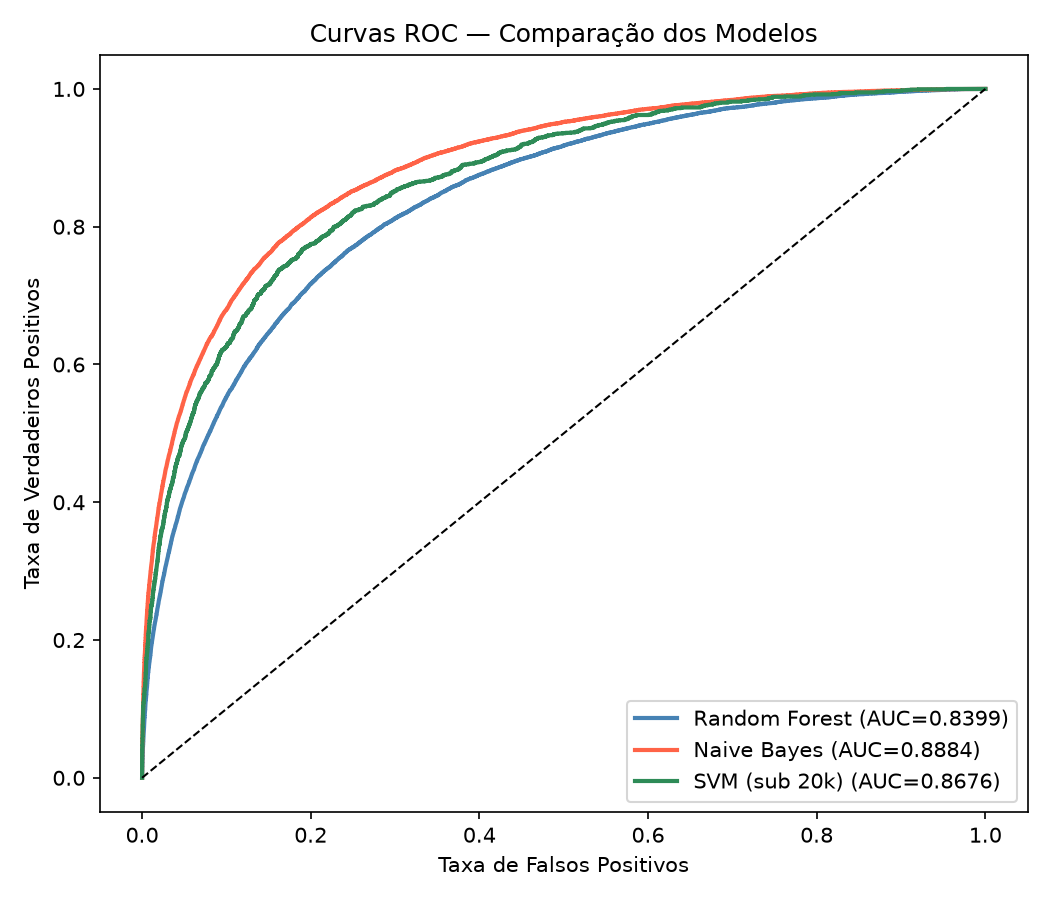
\includegraphics[width=0.75\textwidth]{analise_output/roc_curves.png}
    \caption{Curvas ROC dos três modelos avaliados.}
    \label{fig:roc}
\end{figure}

\subsection{Curvas Precisão-Revocação}

A Figura~\ref{fig:pr} apresenta as curvas Precisão-Revocação. Em dados desbalanceados, essa curva é mais informativa que a ROC, pois foca exclusivamente na classe minoritária. O Naive Bayes apresentou a maior Average Precision (AP = 0,5837), superando os demais modelos.

\begin{figure}[H]
    \centering
    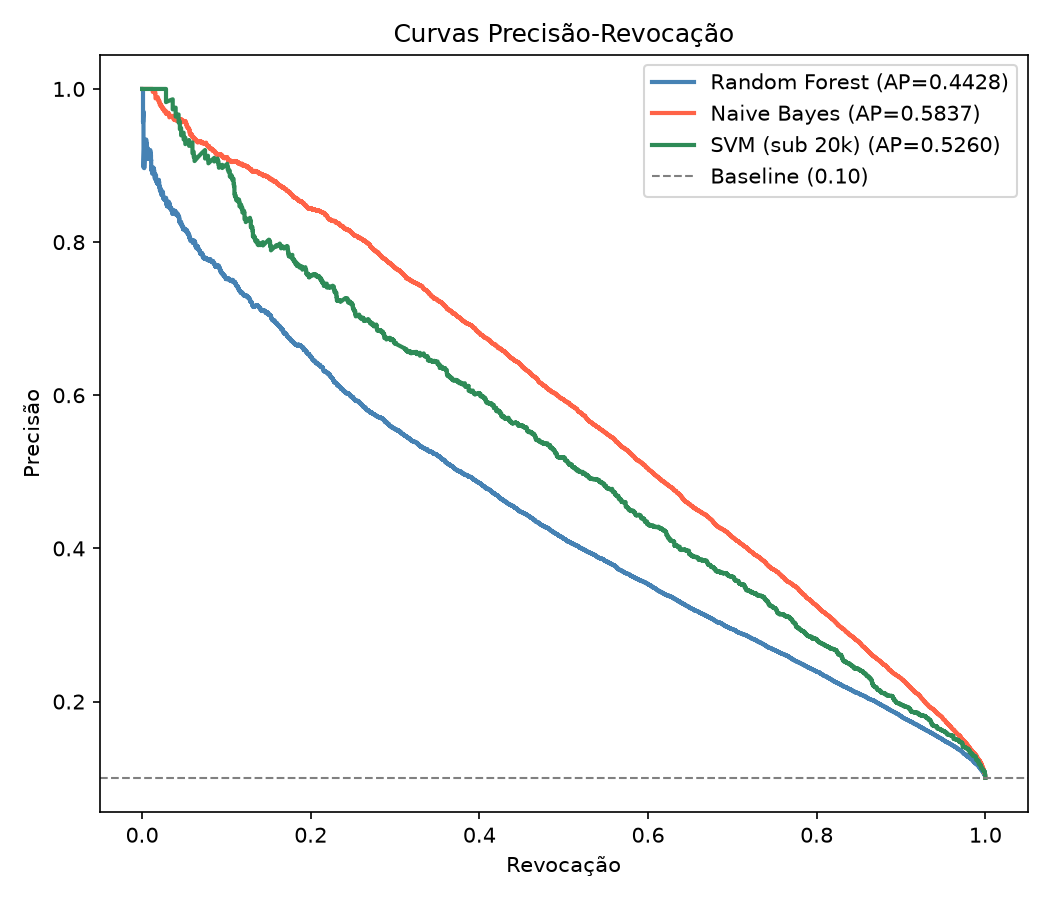
\includegraphics[width=0.75\textwidth]{analise_output/precision_recall_curves.png}
    \caption{Curvas Precisão-Revocação. A linha tracejada representa o baseline (10\% positivo).}
    \label{fig:pr}
\end{figure}

\subsection{Matrizes de confusão}

A Figura~\ref{fig:cm} exibe as matrizes de confusão com limiar de decisão $\theta = 0{,}5$.

\begin{figure}[H]
    \centering
    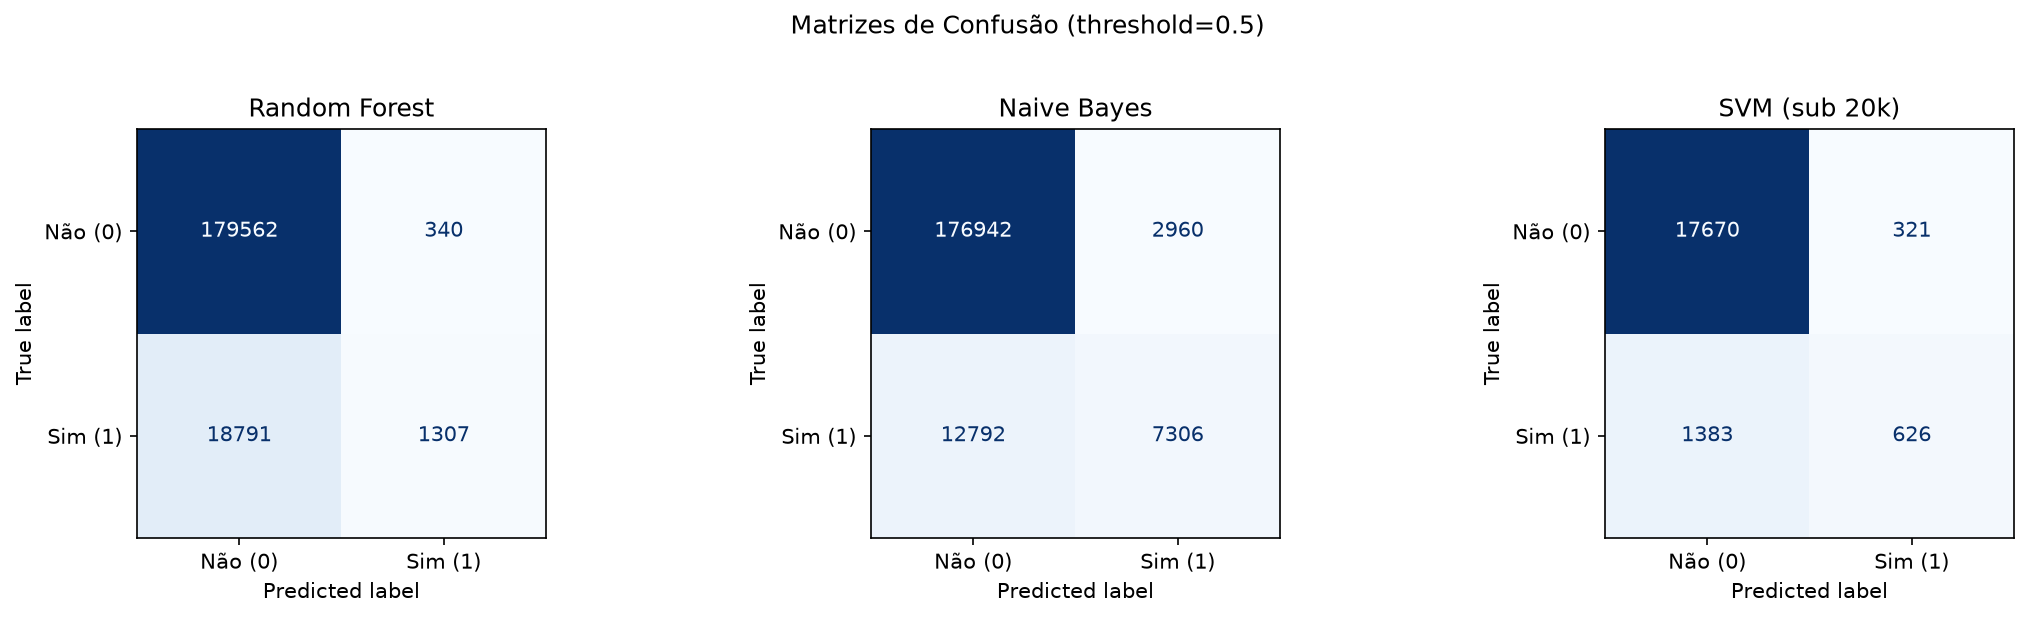
\includegraphics[width=\textwidth]{analise_output/confusion_matrices.png}
    \caption{Matrizes de confusão dos três modelos (limiar = 0,5).}
    \label{fig:cm}
\end{figure}

O Random Forest destaca-se negativamente: com revocação de apenas 6,5\%, detecta muito poucas transações reais (242 de 4.020 no fold final). O Naive Bayes detectou 37\% das transações reais, com menor taxa de falsos negativos.

\subsection{Importância das features — Random Forest}

A Figura~\ref{fig:imp} apresenta as 20 features mais importantes segundo o Random Forest, estimadas pela redução média de impureza nas árvores.

\begin{figure}[H]
    \centering
    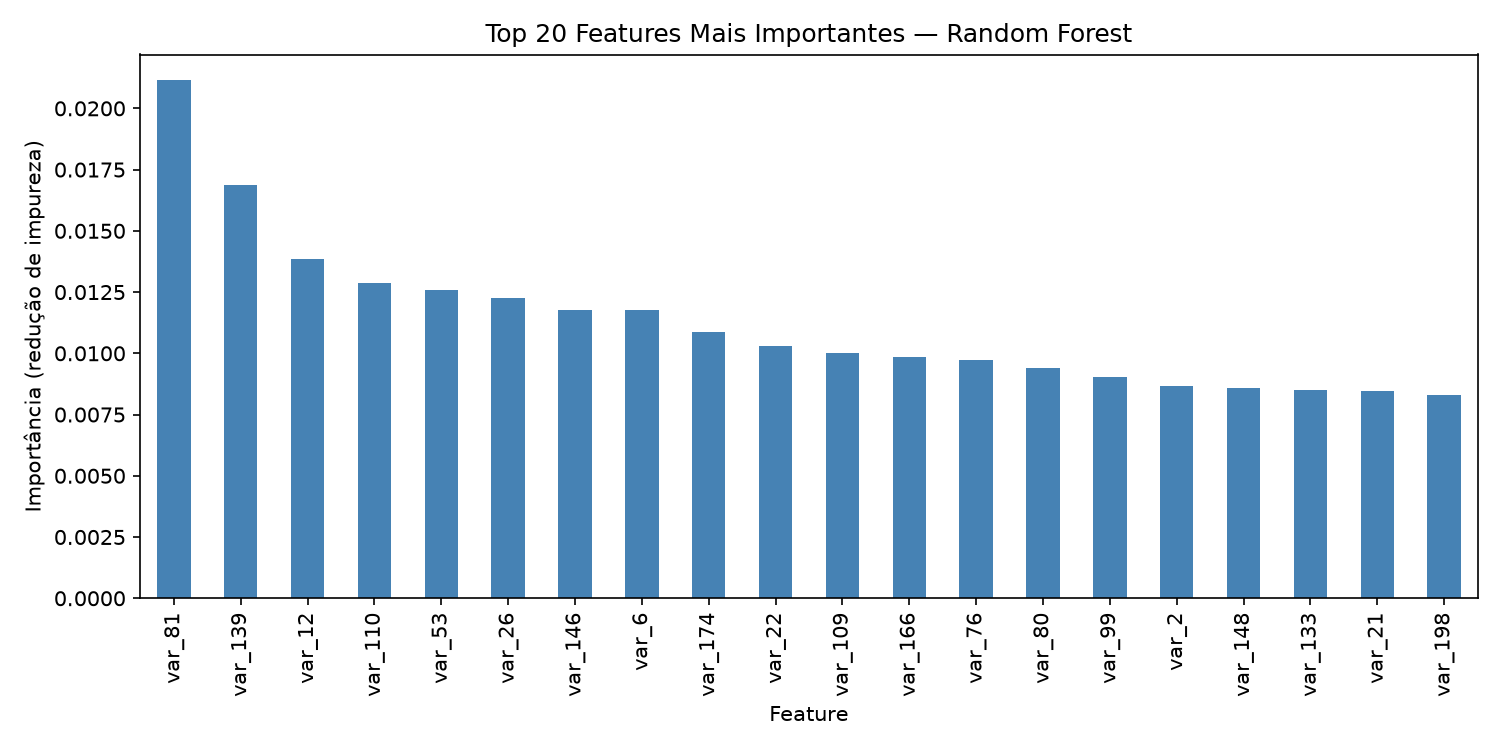
\includegraphics[width=0.85\textwidth]{analise_output/feature_importance.png}
    \caption{Top 20 features mais importantes segundo o Random Forest.}
    \label{fig:imp}
\end{figure}

As features \texttt{var\_81}, \texttt{var\_139} e \texttt{var\_12} foram as mais informativas. A importância está distribuída de forma relativamente uniforme entre as 200 variáveis, indicando que não há um pequeno subconjunto dominante.

\subsection{Distribuição das probabilidades previstas}

A Figura~\ref{fig:prob} mostra a distribuição das probabilidades previstas para cada classe. Um modelo bem calibrado deve apresentar separação clara entre as distribuições de target = 0 e target = 1.

\begin{figure}[H]
    \centering
    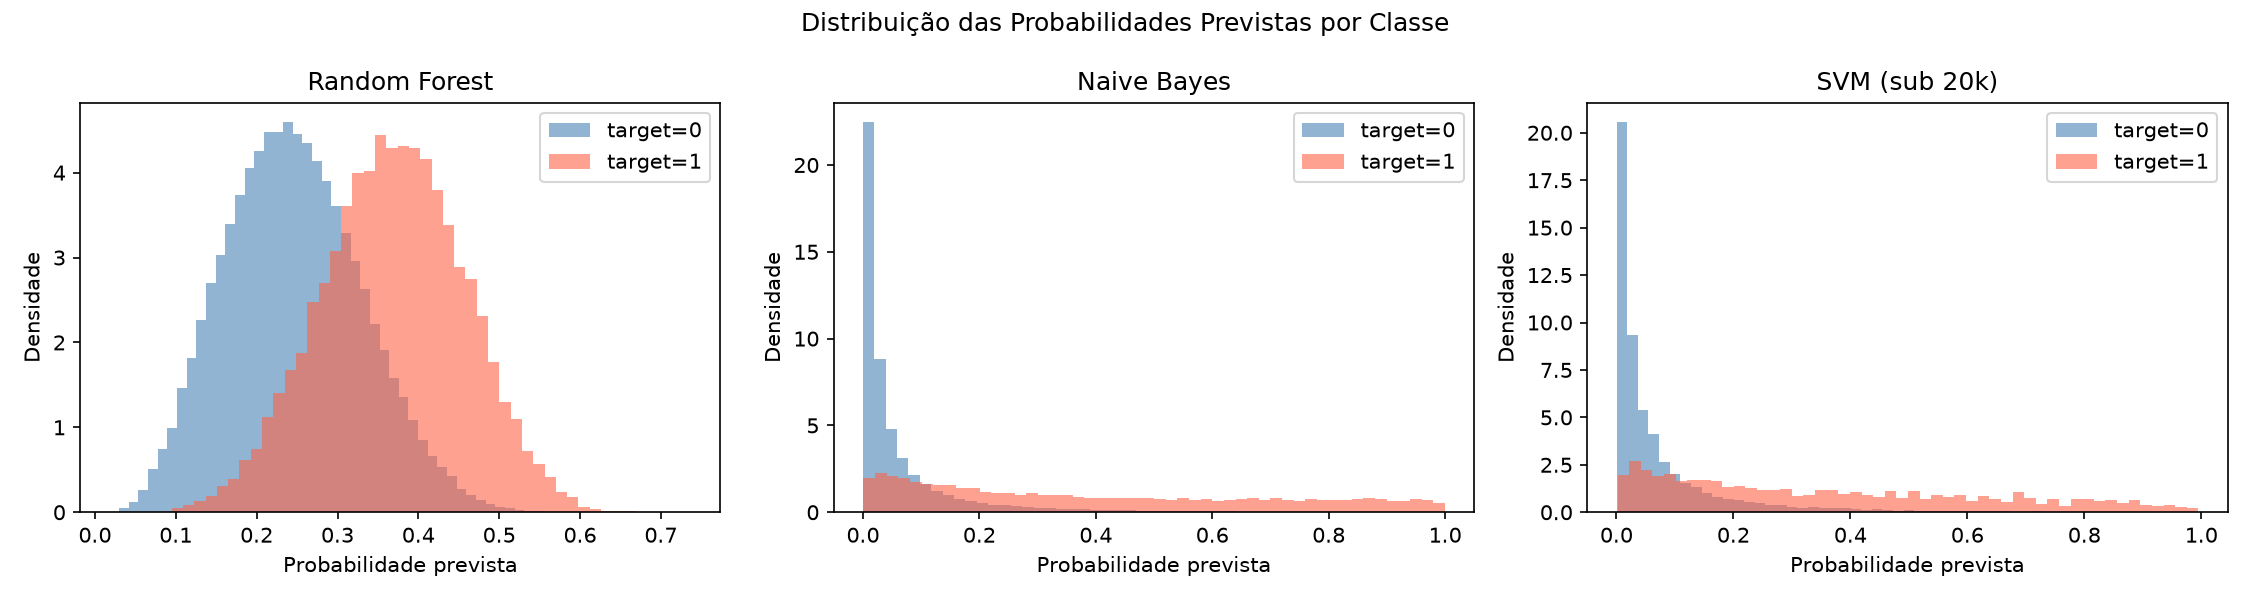
\includegraphics[width=\textwidth]{analise_output/prob_distributions.png}
    \caption{Distribuição das probabilidades previstas por classe e por modelo.}
    \label{fig:prob}
\end{figure}

\newpage

% ----------------------- ANÁLISE E DISCUSSÃO -----------------------
\section{Análise e Discussão}

\subsection{Por que o Naive Bayes superou o Random Forest?}

O resultado mais relevante deste trabalho é a superioridade do Naive Bayes Gaussiano frente ao Random Forest, que contraria a expectativa intuitiva. Isso pode ser explicado pelas características específicas dos dados:

\begin{itemize}
    \item As 200 features são anônimas e sem estrutura semântica conhecida, sugerindo baixa correlação entre elas. Esse cenário favorece a suposição de independência do Naive Bayes;
    \item O Random Forest, ao dividir o espaço de features aleatoriamente, dilui o sinal de cada variável ao longo das árvores. Com 200 features de baixa importância individual, o método perde eficiência discriminativa;
    \item O Naive Bayes combina o sinal de todas as 200 features de forma aditiva (no espaço logarítmico), aproveitando melhor a contribuição coletiva de variáveis fracamente informativas.
\end{itemize}

\subsection{Limitações do SVM}

O SVM com kernel RBF apresentou AUC de 0,8676 dentro da subamostra de 20.000 amostras. Contudo, esse resultado não é diretamente comparável aos demais modelos, pois foi treinado em apenas 10\% dos dados. Em teoria, com mais dados, o SVM poderia apresentar desempenho superior, mas o custo computacional $O(n^2)$ inviabiliza o treino no conjunto completo sem hardware especializado.

\subsection{Relevância das métricas para o problema}

Em um problema de detecção de transações, a revocação (capacidade de encontrar transações reais) é tão importante quanto a precisão (evitar falsos alarmes). O Random Forest, com revocação de apenas 6,5\%, seria pouco útil em produção apesar de sua alta acurácia geral. O Naive Bayes equilibra melhor esses aspectos, com F1-score de 0,4812 na classe positiva, contra apenas 0,1202 do Random Forest.

\newpage

% ----------------------- CONCLUSÃO -----------------------
\section{Conclusão}

Este trabalho desenvolveu e comparou três modelos de classificação binária aplicados ao problema de predição de transações bancárias do desafio Santander Customer Transaction Prediction. Os modelos implementados seguiram as técnicas abordadas em aula, com pré-processamento por padronização, tratamento do desbalanceamento e validação cruzada estratificada.

O \textbf{Naive Bayes Gaussiano} obteve o melhor desempenho, com AUC-ROC de 0,8884 e F1-score de 0,4812 na classe positiva, superando o Random Forest (AUC = 0,8399) e o SVM (AUC = 0,8676 em subamostra). A superioridade do Naive Bayes está associada à natureza do conjunto de dados: 200 features anônimas com baixa correlação entre si favorecem a suposição de independência condicional do modelo.

Conclui-se que a escolha adequada do algoritmo depende das características dos dados, não apenas da complexidade do modelo. Em conjuntos de alta dimensionalidade com features fracamente correlacionadas, modelos probabilísticos simples podem superar métodos mais sofisticados como Random Forest.

\end{document}
